\section{Durchführung}
\label{sec:Durchfuehrung}
Um mit dem Lock-In-Verstärker vertraut zu werden, werden vor eigentlichem Versuchsbeginn nacheinander die beiden Ausgänge des Funktionengenerators an das bereitstehende Oszilloskop geschlossen. 
Durch Ausprobieren kann festgestellt werden, welches das zu messende Signal bzw. das Referenzsignal ist.
Die Amplitude des Referenzsignals kann im Gegensatz zum Messsignal verändert werden; 
außerdem besteht die Möglichkeit zwischen Rechteck- und Sinusspannung zu wählen.
\begin{figure}
	\centering
	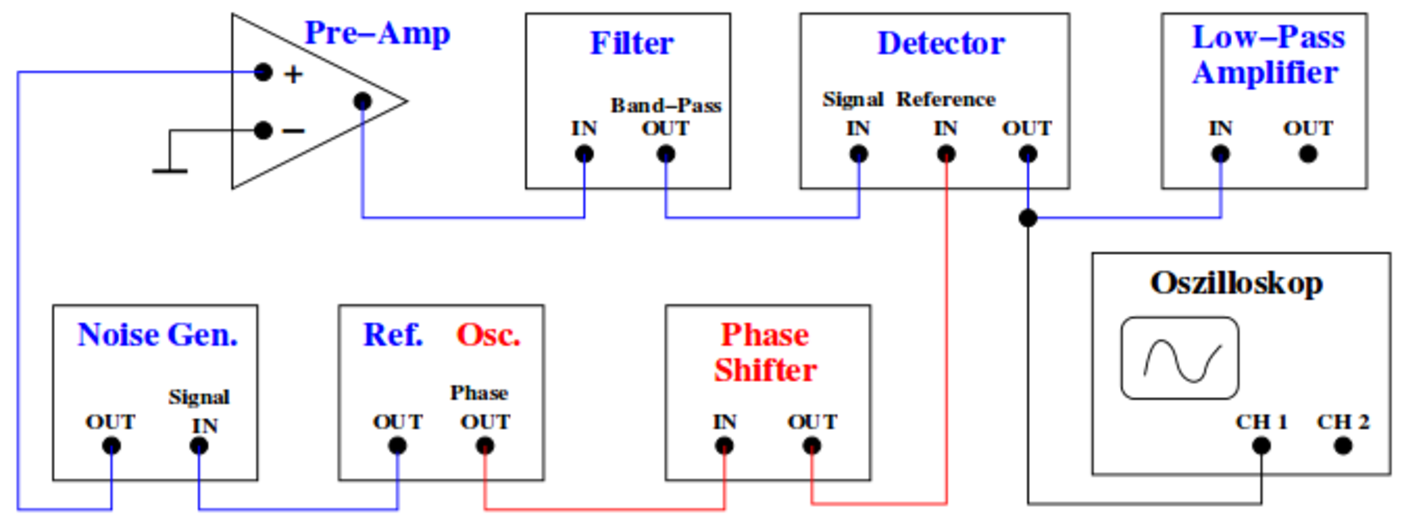
\includegraphics[width=0.7\textwidth]{Bilder/Messung1.pdf}	
	\caption{Schematischer Versuchsaufbau zur Verifizierung der Funktionsweise des Verstärkers. \cite{V303}}
	\label{fig:M1}	
\end{figure}

Im ersten Versuchsteil soll die Funktionsweise des Gerätes bestätigt werden. 
Dazu wird die in Abbildung \ref{fig:M1} gezeigte Schaltung aufgebaut. 
Der Noise-Generator wird in diesem Versuchsteil nicht benötigt und für die Messung überbrückt. 
Es werden Frequenz und Amplitude des Mess- und des sinusförmigen Referenzsignals eingestellt. 
Mit dem Phasenschieber werden 10 unterschiedliche Phasen realisiert und die Werte der Ausgangsspannung notiert.

Dieser Vorgang wird anschließend mit verrauschtem Sinussignal wiederholt. 
Dazu wird der vorher überbrückte Noise-Generator zugeschaltet.

\begin{figure}
	\centering
		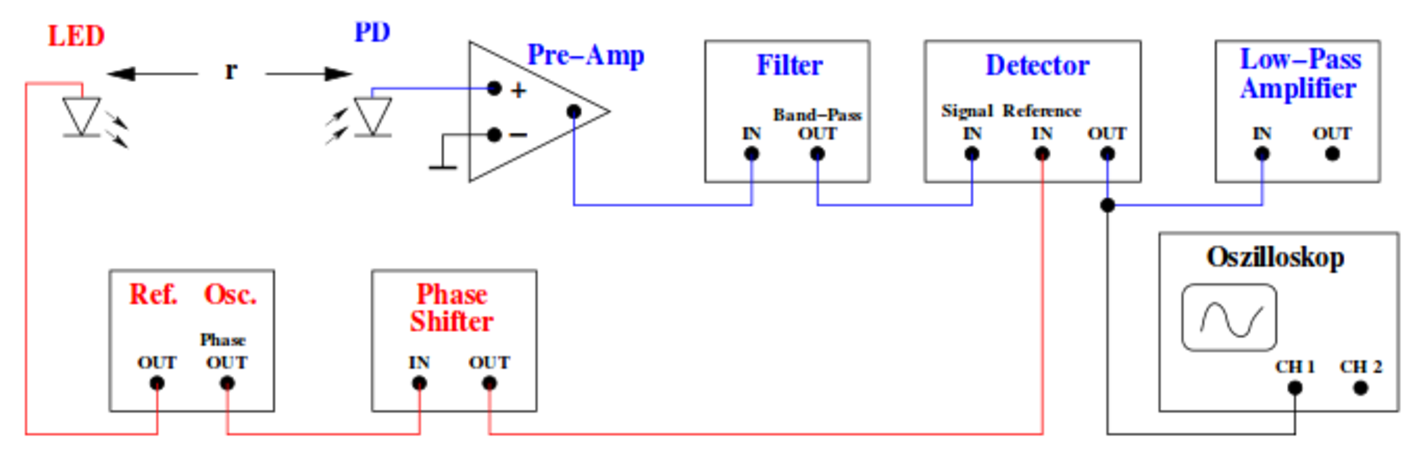
\includegraphics[width=0.7\textwidth]{Bilder/Messung2.pdf}
		\caption{Versuchsaufbau zur Messung mit Photodiode. \cite{V303}}
		\label{fig:M2}
	\end{figure}

Die in Abbildung \ref{fig:M2} skizzierte Schaltung wird im zweiten Versuchsteil aufgebaut. 
Der Noise-Generator wird nun durch eine LED, sowie der dazugehörigen Photodiode ersetzt. 
Es soll die Intensität des Lichtes eines gepulsten LED-Signales in Abhängigkeit vom Abstand gemessen werden.
Die sich auf einer Metallschiene befindliche LED soll mit einer Frequenz von \SI{300}{\hertz} blinken, was mit einer Rechteckspannung gleicher Frequenz realisiert wird. 
Nach Verschieben der Photodiode auf der Metallschiene kann die Ausgangsspannung am Lock-In-Verstärker abgelesen werden.
Das Oszilloskop dient dazu, die verschiedenen Signale sichtbar zu machen. 
Es kann beliebig an die verschiedenen Bestandteile des Verstärkers angeschlossen werden. 
%Außerdem besteht die Möglichkeit, Screenshots der auf dem Bildschirm dargestellten Signale anzufertigen und auf einem USB-Stick zu speichern.
